\documentclass[pdf, 9pt, fleqn, handout]{beamer}

\usepackage[utf8]{inputenc}
\usepackage[english]{babel}
\usepackage{csquotes}

\usepackage{amsmath}
\usepackage{amssymb}
\usepackage{mathtools}
\usepackage{array}
\usepackage{bm}
\usepackage{graphicx}
\usepackage{etoolbox}
\usepackage{amsthm}
\usepackage{tikz}
\usepackage{verbatim}
\usetikzlibrary{arrows}
\usetikzlibrary{arrows.meta}
\usepackage{xcolor}

\newenvironment{myitemize}
{\begin{itemize}
  \setlength{\itemsep}{0pt}
  \setlength{\parskip}{7pt}
  \setlength{\parsep}{0pt}}
{\end{itemize}}

\usecolortheme{Fjelstul}
\usepackage[scaled]{helvet}

\definecolor{darkblue}{HTML}{2980b9}

\setlength{\mathindent}{5pt}

\makeatother
\setbeamertemplate{footline}
{
  \leavevmode
  \hbox{%
  \begin{beamercolorbox}[wd=.5\paperwidth,ht=3ex,dp=2ex,center]{author in head/foot}
    \usebeamerfont{author in head/foot}\insertshortauthor
  \end{beamercolorbox}%
  \begin{beamercolorbox}[wd=.5\paperwidth,ht=3ex,dp=2ex,center]{title in head/foot}
    \usebeamerfont{title in head/foot}\insertshorttitle
  \end{beamercolorbox}}
  \vskip0pt
}
\makeatletter
\setbeamertemplate{navigation symbols}{}

\setbeamersize{text margin left=0.25in, text margin right=0.5in}

\definecolor{gray}{gray}{0.8}

\title[IHEID Text Analysis Workshop]{Social Science Methods for Lawyers: Text Analysis \\[0.5em] A Survey of Text Analysis Methods}
\author[Joshua C. Fjelstul, Ph.D.]{Joshua C. Fjelstul, Ph.D.}
\institute{Post-Doctoral Research Fellow, University of Geneva \\[0.5em] Researcher, ARENA Centre for European Studies, University of Oslo}
\date{}

\begin{document}

\maketitle

\begin{frame}{What are we going to cover in this workshop?}
\begin{itemize}
\item What is text analysis? What methods does it include? \\[1em]
\item How does text analysis relate to statistics, machine learning (ML), and natural language processing (NLP)? \\[1em]
\item How can we use text analysis to study international legal texts? \\[1em]
\item How can we implement some basic text analysis tools in R?
\end{itemize}
\end{frame}

\begin{frame}{What is quantitative text analysis?}
\begin{itemize}
\item Quantitative text analysis is the use of quantitative methods to analyze the content of documents
\end{itemize}
\end{frame}

\begin{frame}{Levels of analysis}
\begin{itemize}
\item Corpus \\[1em]
\item Documents  \\[0.5em]
\begin{itemize}
\item Books, documents, judgments, speeches, tweets  \\[1em]
\end{itemize}
\item Paragraphs  \\[1em]
\item Sentences  \\[1em]
\item Words
\end{itemize}
\end{frame}

\begin{frame}{Assumptions}
\begin{itemize}
\item The content of text reveals something meaningful and interesting about the author that we can use to answer research questions \\[1em]
\item Text can be represented by features (words, lemmas, $n$-grams) \\[1em]
\item The relative distribution of words in documents captures meaningful variation in topics and substantively important latent dimensions \\[0.5em]
\begin{itemize}
\item We make a matrix called a document feature matrix (DFM) with words in columns, documents in rows, and frequencies in cells that describe these distributions \\[1em]
\item This might seem unsatisfactory \\[1em]
\item Some kinds of neural networks can take into account word order \\[1em]
\item Taking into account word order adds a lot of complexity but doesn't usually change things much
\end{itemize}
\end{itemize}
\end{frame}

\begin{frame}{Types of quantitative text analysis}
\begin{itemize}
\item Frequency analysis\\[0.5em]
\begin{itemize}
\item What words/tokens are important? \\[0.5em]
\item Descriptive \\[1em]
\end{itemize}
\item Similarity\\[0.5em]
\begin{itemize}
\item How similar are documents/paragraphs/sentences?  \\[0.5em]
\item Descriptive  \\[1em]
\end{itemize}
\item Scaling\\[0.5em]
\begin{itemize}
\item How do documents/paragraphs/sentences compare on a continuous latent dimension?  \\[0.5em]
\item Inferential (statistical models, machine learning models)  \\[1em]
\end{itemize}
\item Classification\\[0.5em]
\begin{itemize}
\item How do documents/paragraphs/sentences cluster into discrete groups? \\[0.5em]
\item Inferential (statistical models, machine learning models)  \\[1em]
\end{itemize}
\end{itemize}
\end{frame}

\begin{frame}{Natural language processing (NLP)}
\begin{itemize}
\item Text analysis overlaps with NLP — using computers to process and analyze language \\[0.5em]
\begin{itemize}
\item Language processing \\[0.5em]
\begin{itemize}
\item Optical character recognition (OCR) \\[0.5em]
\item Speech recognition \\[0.5em]
\end{itemize}
\item Morphology \\[0.5em]
\begin{itemize}
\item Lemmatization \\[0.5em]
\item Stemming \\[0.5em]
\item Part-of-speech (POS) tagging \\[0.5em]
\end{itemize}
\item Semantics \\[0.5em]
\begin{itemize}
\item Sentiment analysis \\[0.5em]
\item Named entity recognition \\[0.5em]
\item Word-sense disambiguation \\[0.5em]
\end{itemize}
\item High-level tasks \\[0.5em]
\begin{itemize}
\item Machine translation \\[0.5em]
\item Natural language generation \\[0.5em]
\item Question answering 
\end{itemize}
\end{itemize}
\end{itemize}
\end{frame}

\begin{frame}{Machine learning (ML)}
\begin{itemize}
\item Machine learning is the use of algorithms to predict outcomes based on data \\[2em]
\item Algorithms learn the relationship between input data and labels based on training data and then make predictions for unseen data \\[2em]
\item Quantitative text analysis is an application of ML to text data
\end{itemize}
\end{frame}

\begin{frame}{Learning}
\begin{itemize}
\item Supervised learning \\[0.5em]
\begin{itemize}
\item Train a scaling/classification model on a pre-defined dimension using pre-coded training data \\[2em]
\end{itemize}
\item Unsupervised learning \\[0.5em]
\begin{itemize}
\item Train a scaling/classification model to endogenously learn an underlying dimension or categories using training data
\end{itemize}
\end{itemize}
\end{frame}

\begin{frame}{Learning}
\begin{itemize}
\item Supervised learning \\[0.5em]
\begin{itemize}
\item Advantages \\[0.5em]
\begin{itemize}
\item You already know the topics/dimensions so you know how to interpret your estimates \\[0.5em]
\end{itemize}
\item Disadvantages \\[0.5em]
\begin{itemize}
\item It requires labeled training data (a lot of work) \\[0.5em]
\item You have to know ahead of time what the relevant topics/dimensions are \\[1em]
\end{itemize}
\end{itemize}
\item Unsupervised learning \\[0.5em]
\begin{itemize}
\item Advantages \\[0.5em]
\begin{itemize}
\item You can explore naturally occurring topics and primary latent dimensions \\[0.5em]
\item You don't have to create labeled training data \\[0.5em]
\end{itemize}
\item Disadvantages \\[0.5em]
\begin{itemize}
\item You have to validate that the topics/dimensions you uncover are meaningful and you have to figure out how to interpret them \\[0.5em]
\item You might not find meaningful topics/dimensions (or the ones you expect) \\[0.5em]
\item Unsupervised methods are harder to learn
\end{itemize}
\end{itemize}
\end{itemize}
\end{frame}

\begin{frame}{Parametric vs non-parametric models}
\begin{itemize}
\item Scaling and classification models can be parametric or non-parametric \\[2em]
\item Parametric models overlap with statistics and involve estimating the values of parameters that you can interpret to learn about the content of documents \\[2em]
\item Non-parametric methods overlap with machine learning and depend on complex algorithms to learn the relationship between text data and labels
\end{itemize}
\end{frame}

\begin{frame}{Classification}
\begin{itemize}
\item Supervised methods for text \\[0.5em]
\begin{itemize}
\item Naive Bayes classifier (non-parametric) \\[0.5em]
\item Regression classifiers (parametric) \\[0.5em]
\item Random forests (non-parametric) \\[0.5em]
\item Neural networks (non-parametric) \\[0.5em]
\item Support vector machines (SVM) (non-parametric) \\[2em]
\end{itemize}
\item Unsupervised methods for text \\[0.5em]
\begin{itemize}
\item Latent Dirichlet allocation (LDA) (parametric) \\[0.5em]
\item Seeded LDA  (parametric) \\[0.5em]
\item Structural topic models (STM) (parametric)
\end{itemize} 
\end{itemize}
\end{frame}

\begin{frame}{Scaling}
\begin{itemize}
\item Supervised \\[0.5em]
\begin{itemize}
\item Wordscores \\[3em]
\end{itemize}
\item Unsupervised \\[0.5em]
\begin{itemize}
\item Correspondence analysis (non-parametric) (dimensionality reduction) \\[1em]
\item Latent semantic analysis (non-parametric) (dimensionality reduction) \\[1em]
\item Wordfish (parametric)
\end{itemize}
\end{itemize}
\end{frame}

\begin{frame}{Topic models}
\begin{itemize}
\item Topics models are unsupervised methods for identifying naturally occurring topics in documents \\[1em]
\item The most common type of topic model is latent Dirichlet allocation (LDA) \\[1em]
\item It assumes that documents are mixtures of topics and that topics are mixtures of words \\[1em]
\item Documents are not sorted into discrete categories \\[1em]
\item A topic is a distribution of words \\[1em]
\item The goal is to figure out which words are associated with which topics and which topics make up each document
\end{itemize}
\end{frame}

\begin{frame}{Topic models}
\begin{itemize}
\item You have to tell the model how many topics to find \\[1em]
\item You can look at the words that are most strongly associated with each topic \\[1em]
\item Based on that list of words, we can label each topic \\[1em]
\item Some topics will be more distinct that others \\[1em]
\item If topics overlap too much, we may need fewer topics \\[1em]
\item It topics are not distinct, we may need more topics \\[1em]
\item The model estimates the probability that each topic applies to each document
\end{itemize}
\end{frame}

\begin{frame}{Word scores}
\begin{itemize}
\item Supervised scaling method \\[1em]
\item You start with a set of reference texts \\[1em]
\item These need to represent the two poles of your latent dimension \\[1em]
\item The reference texts are like a training set \\[1em]
\item You calculate word scores based on the reference text and then use them to score the rest of the texts \\[1em]
\item Each document will have a single score that represents its position on the latent dimension
\end{itemize}
\end{frame}

\begin{frame}{Word scores}
\begin{itemize}
\item  Advantages \\[0.5em]
\begin{itemize}
\item After you choose the reference text, it's fully automated \\[1em]
\item It scales all documents between the references texts at each end of the dimension \\[3em]
\end{itemize}
\item Disadvantages \\[0.5em]
\begin{itemize}
\item It really matters which documents you use as the reference texts \\[1em]
\item The dimension you define by choosing the reference texts may not be the dimension that explains the most variation in the content of your documents \\[1em]
\item It's hard to choose the most extreme documents without a lot of knowledge about the content of documents (hard when there are a lot) 
\end{itemize}
\end{itemize}
\end{frame}

\begin{frame}{Wordfish (intuition)}
\begin{itemize}
\item Unsupervised scaling method \\[1em]
\item The input data is a DFM \\[1em]
\item We don't have to know the underlying dimension ahead of time \\[1em]
\item So we have to show that our estimates capture a meaningful latent dimension \\[1em]
\item Based on a poison distribution \\[0.5em]
\begin{itemize}
\item The poisson distribution models counts of discrete events — like the occurrence of words in a document \\[1em]
\item Wordfish is a type of poisson scaling model
\end{itemize}
\end{itemize}
\end{frame}

\begin{frame}{Wordfish (equation)}
\begin{itemize}
\item The model equation is:
\begin{align*}
log \lambda_{ij} = \alpha_i + \theta_i \beta_j + \phi_j
\end{align*}
\item Parameters: \\[0.5em]
\begin{itemize}
\item $\lambda_{ij}$ is the expected frequency of a word $i$ in document $j$ \\[0.5em]
\item $i$ indexes documents \\[0.5em]
\item $j$ indexes words \\[0.5em]
\item $\theta_i$ is the latent position of document $i$ that we want to estimate \\[0.5em]
\item $\beta_j$ is the latent position of word $j$ (the strong of the relationship between the latent dimension and the frequency) \\[0.5em]
\item $\alpha_i$ is a document fixed effect (controls for how long each document is) \\[0.5em]
\item $\phi_j$ is a word fixed effect (controls for how common/rare each word is) \\[1em]
\end{itemize}
\item We can estimate standard errors and construct confidence intervals for each parameter to express uncertainty, just like with a regression model
\end{itemize}
\end{frame}

\begin{frame}{Wordfish (estimation)}
\begin{itemize}
\item On the right-hand side of a regression equation, we have data and parameters \\[1em]
\item The data is constant and we estimate the parameters \\[1em]
\item But here, there's no data on the right-hand side, so what do we do? \\[0.5em]
\begin{itemize}
\item We start with random values for all of the parameters \\[0.5em]
\item We hold $\phi$ and $\beta$ (the word parameters) constant and estimate $\alpha$ and $\theta$ (the document parameters) \\[0.5em]
\item Then we hold $\alpha$ and $\theta$ (the document parameters) constant and estimate $\phi$ and $\beta$ (the word parameters) \\[0.5em]
\item And we iterate back and forth \\[0.5em]
\item This is called expectation-maximization \\[0.5em]
\item Eventually, we'll converge to good estimates of all parameters
\end{itemize}
\end{itemize}
\end{frame}

\begin{frame}{Wordfish (interpretation)}
\begin{itemize}
\item We can interpret the $\theta$ estimates as the position of each document on our latent dimension. This is the main thing we're interested in \\[1em]
\item But this is an unsupervised model, so how do we know what the latent dimension is? \\[0.5em]
\begin{itemize}
\item We can plot the word fixed effects (y-axis) against the word positions (x-axis) to get an idea of what the dimension is \\[1em]
\item Rarer words (lower fixed effect) will be more discriminatory (will provide more information about how documents differ) \\[1em]
\item Words with more extreme positions (x-axis) will define the substantive content of each pole of the latent dimension \\[1em]
\item You have to convince your audience that your latent dimension is meaningful and interesting
\end{itemize}
\end{itemize}
\end{frame}

\begin{frame}{Wordfish (word positions)}
\begin{figure}
\centering
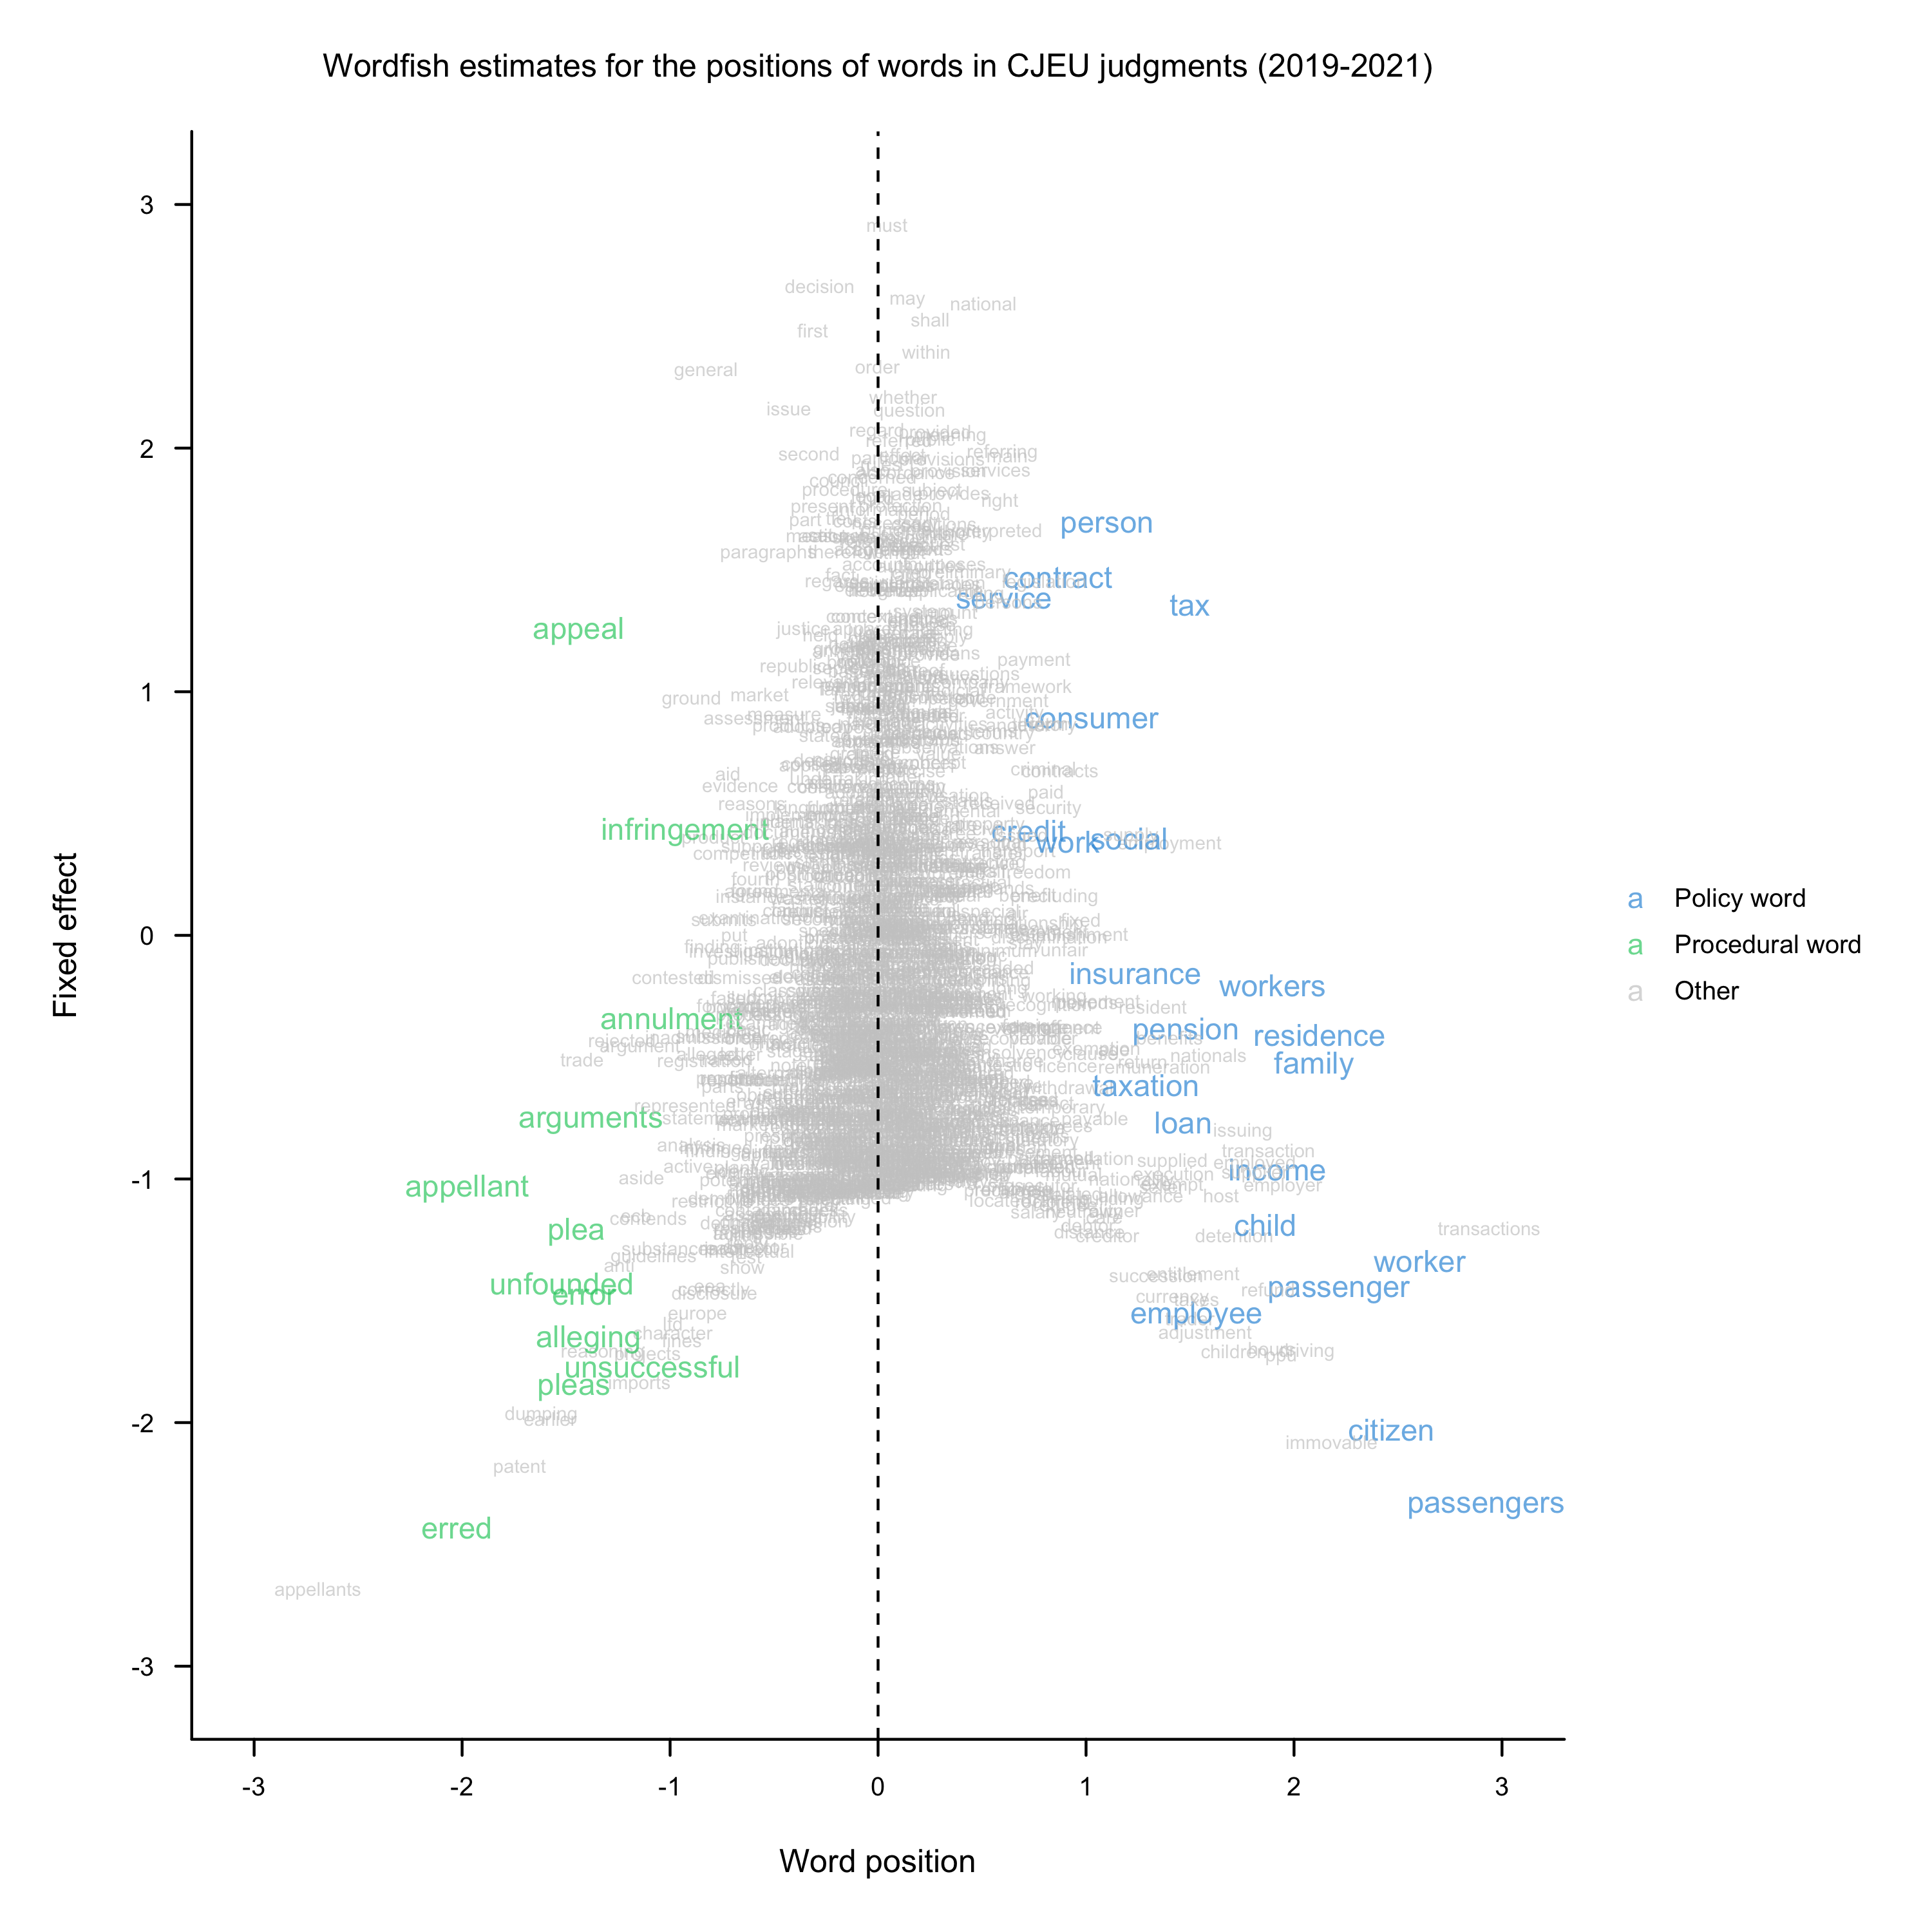
\includegraphics[width = 3in]{word_positions}
\end{figure}
\end{frame}

\begin{frame}{Wordfish (document positions)}
\begin{figure}
\centering
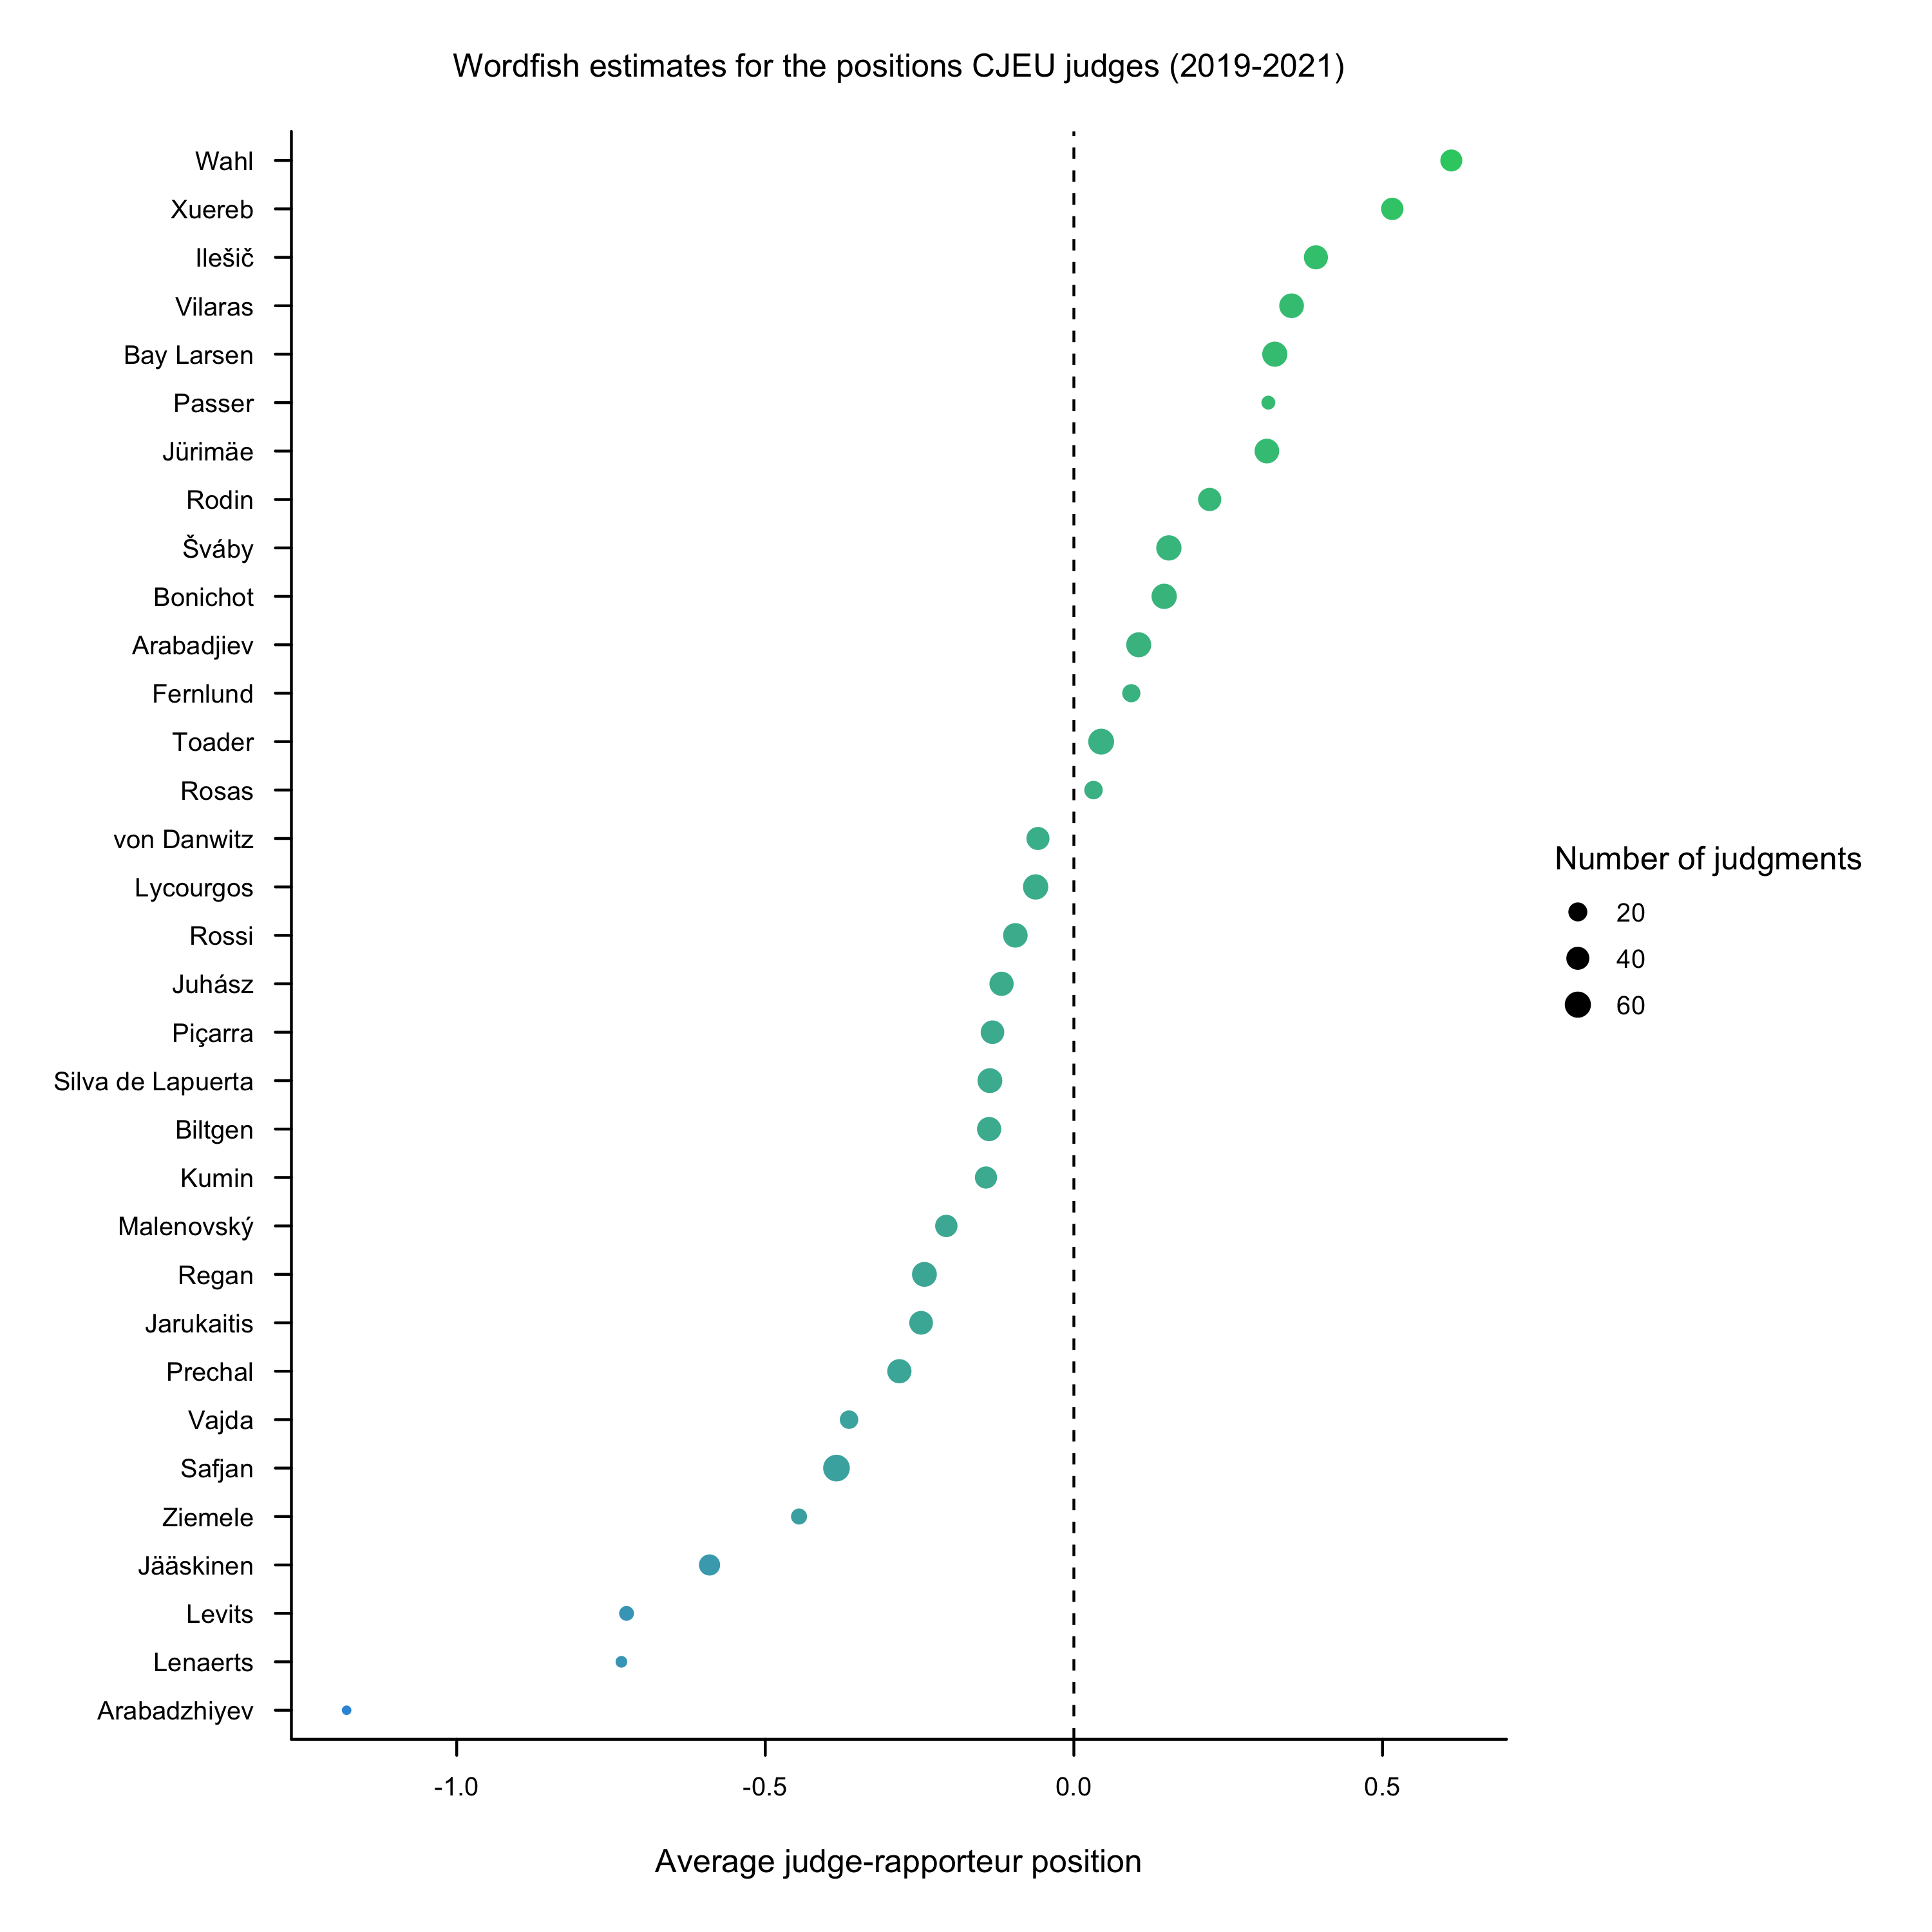
\includegraphics[width = 3in]{judge_positions}
\end{figure}
\end{frame}

\begin{frame}{Research questions}
\begin{itemize}
\item We'll answer two research questions about the content of judgments delivered by the Court of Justice of the European Union (CJEU) \\[0.5em]
\begin{itemize}
\item To what extent do judges specialize in certain areas of law? \\[1em]
\item What is the primary latent dimension in CJEU judgments? Is it a left/right dimension? Is it a pro-/anti-European integration dimension? Or is it something else, like a policy/procedure dimension? \\[3em]
\end{itemize}
\item We'll use unsupervised and semi-supervised topic models to address the first question and an unsupervised scaling model to address the second question
\end{itemize}
\end{frame}

\end{document}
